%%%%%%%%%%%%%%%%%%%%%%%%%%%%%%%%
\chapter{数値実験}\label{Experiment}
%%%%%%%%%%%%%%%%%%%%%%%%%%%%%%%%

% 数値実験の結果を書いてね\chapter{数値実験}
%%%%%%%%%%%%%%%%%%%%%%%%%%%%%%%%%%%%%%%%%%%%%%%%%%%%%%%%%%
                        %第五章%     %数値実験%
%%%%%%%%%%%%%%%%%%%%%%%%%%%%%%%%%%%%%%%%%%%%%%%%%%%%%%%%%%
% \(lambda\)の値を変更\\
% \(N=40\)で実行\\
% \cite{kv}はkvライブラリの説明で引用
前節までの内容をもとに，以下の環境で数値実験を行った．

\begin{itemize}
  \item OS:Ubuntu20.04
  \item プロセッサ: 12th Gen Intel(R) Core(TM) i7-12700   2.10 GHz
  \item コンパイラ:g++ 9.4.0
  \item ソフトウェア:kvライブラリ kv-0.4.57\cite{kv}
  \item ソフトウェア:VCP Library  Alpha 0.1.1\cite{vcp}
\end{itemize}
実験では，Legendre基底の次数を\(N=40\)で固定したまま，\(\alpha=0.25,\beta=1.25,\gamma=1.0,\delta = 0.2,r=0\)で固定し，\(\epsilon\)を\(0.06\)から\(0.046\)の範囲で変化させた．
得られた近似解をグラフ化し，図\ref{fi:uh_ans0.06}から図\ref{fi:vh_ans0.046}に示した．表\ref{hyou:定数}では近似解に対して得られた埋め込み定数の数値を記載した．
表\ref{hyou:精度保証結果}では近似解に対する\(,R,G\)の精度保証結果を記載した．
表\ref{hyou:数値的検証結果}では，\(K^2RG,\norm{\hat{u}-u^*}_{\tilde{\mathcal{F}}}\)の値を記載した．
また，値はすべて上界を記載した．
表からは，\(\epsilon\)の値を小さくすると近似解と厳密解の誤差\(\norm{\hat{u}-u^*}_{\tilde{\mathcal{F}}}\)の値も大きくなっていることがわかる．
また，\(\epsilon=0.046\)の場合\(K^2RG\leq \frac{1}{2}\)の条件を満たさなくなり，
精度保証が失敗したことがわかる．


\begin{figure}[htbp]
  \begin{minipage}{0.45\hsize}
    \centering
    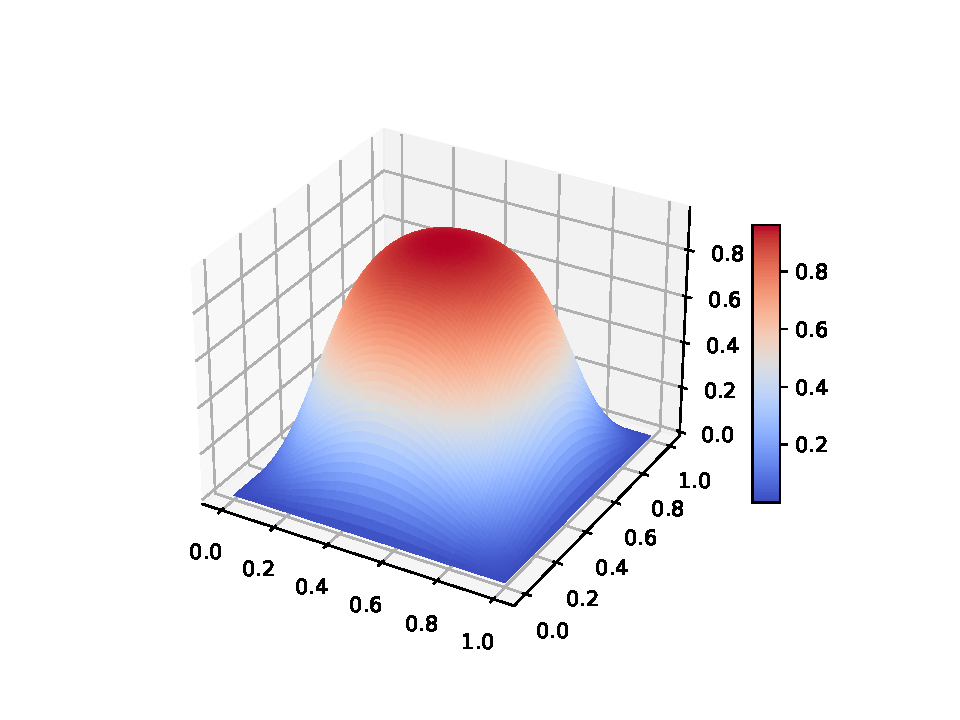
\includegraphics[width=\textwidth,height = 0.8\textwidth ]{true_pic/0.06_uh.pdf}
    \caption{\(\epsilon = 0.06\)の\(\hat{u}\)}
    \label{fi:uh_ans0.06}
  \end{minipage}
  \begin{minipage}{0.45\hsize}
    \centering
    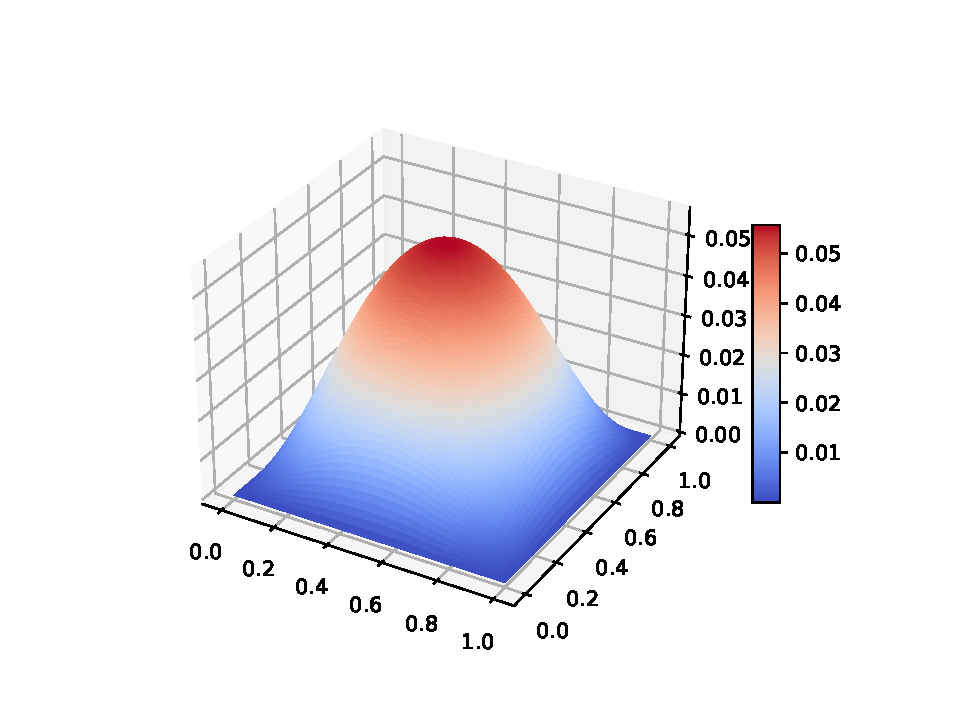
\includegraphics[width=\textwidth,height = 0.8\textwidth ]{true_pic/0.06_vh.pdf}
    \caption{\(\epsilon = 0.06\)の\(\hat{v}\)}
    \label{fi:vh_ans0.06}
  \end{minipage}\\
  \begin{minipage}{0.45\hsize}
    \centering
    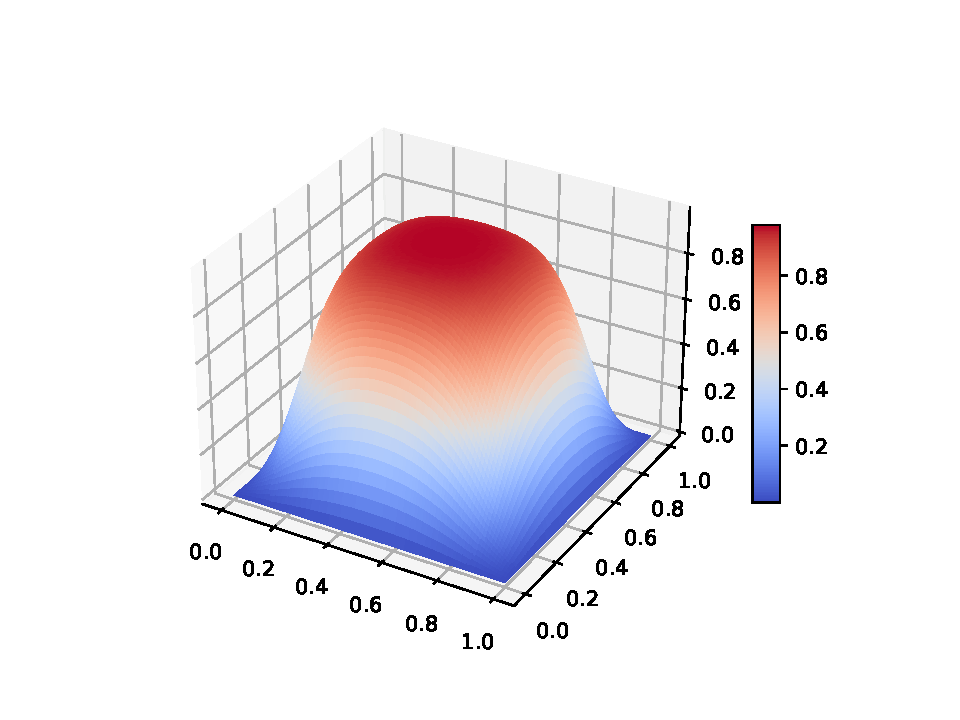
\includegraphics[width=\textwidth,height = 0.8\textwidth ]{true_pic/0.05_uh.pdf}
    \caption{\(\epsilon = 0.05\)の\(\hat{u}\)}
    \label{fi:uh_ans0.05}
  \end{minipage}
  \begin{minipage}{0.45\hsize}
    \centering
    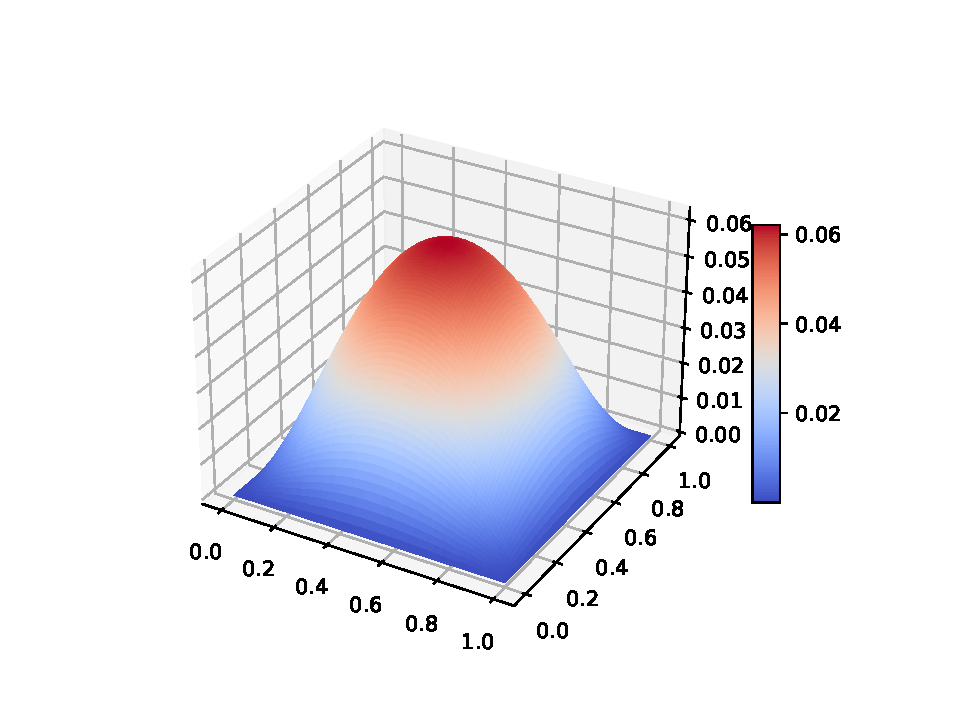
\includegraphics[width=\textwidth,height = 0.8\textwidth ]{true_pic/0.05_vh.pdf}
    \caption{\(\epsilon = 0.05\)の\(\hat{v}\)}
    \label{fi:vh_ans0.05}
  \end{minipage}\\
  \begin{minipage}{0.45\hsize}
    \centering
    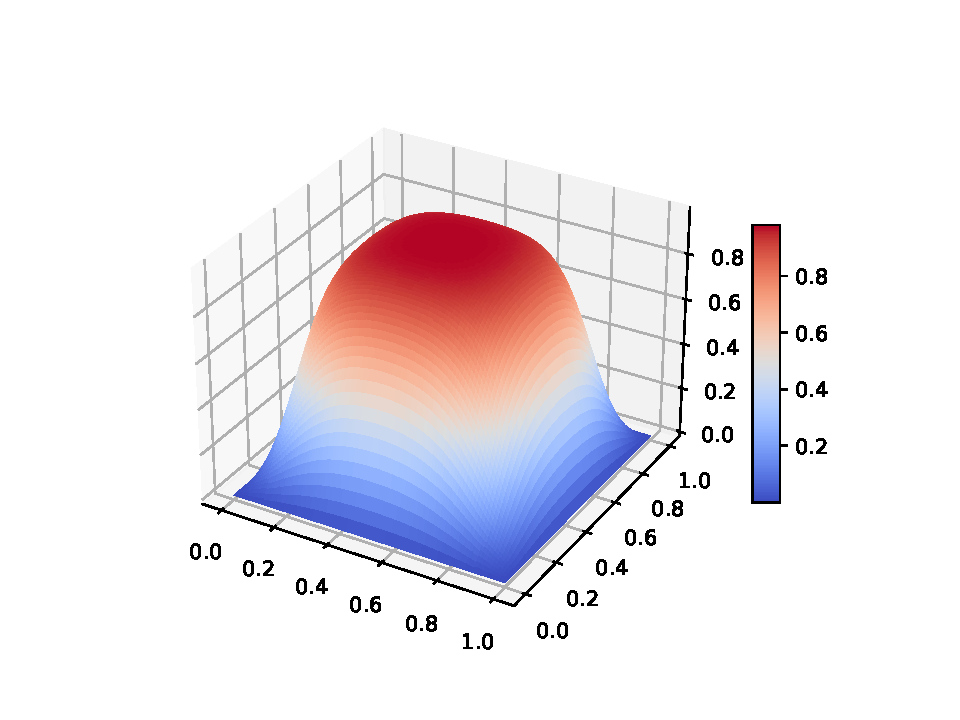
\includegraphics[width=\textwidth,height = 0.8\textwidth ]{true_pic/0.047_uh.pdf}
    \caption{\(\epsilon = 0.047\)の\(\hat{u}\)}
    \label{fi:uh_ans0.047}
  \end{minipage}
  \begin{minipage}{0.45\hsize}
    \centering
    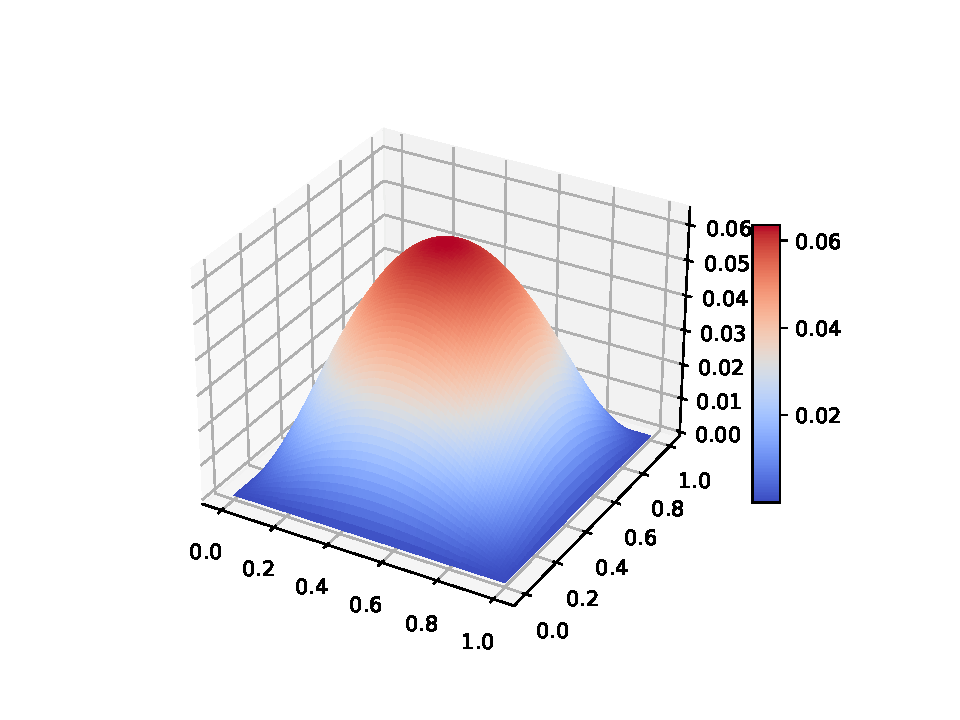
\includegraphics[width=\textwidth,height = 0.8\textwidth ]{true_pic/0.047_vh.pdf}
    \caption{\(\epsilon = 0.047\)の\(\hat{v}\)}
    \label{fi:vh_ans0.047}
  \end{minipage}\\
\end{figure} 
\begin{figure}
  \begin{minipage}{0.45\hsize}
    \centering
    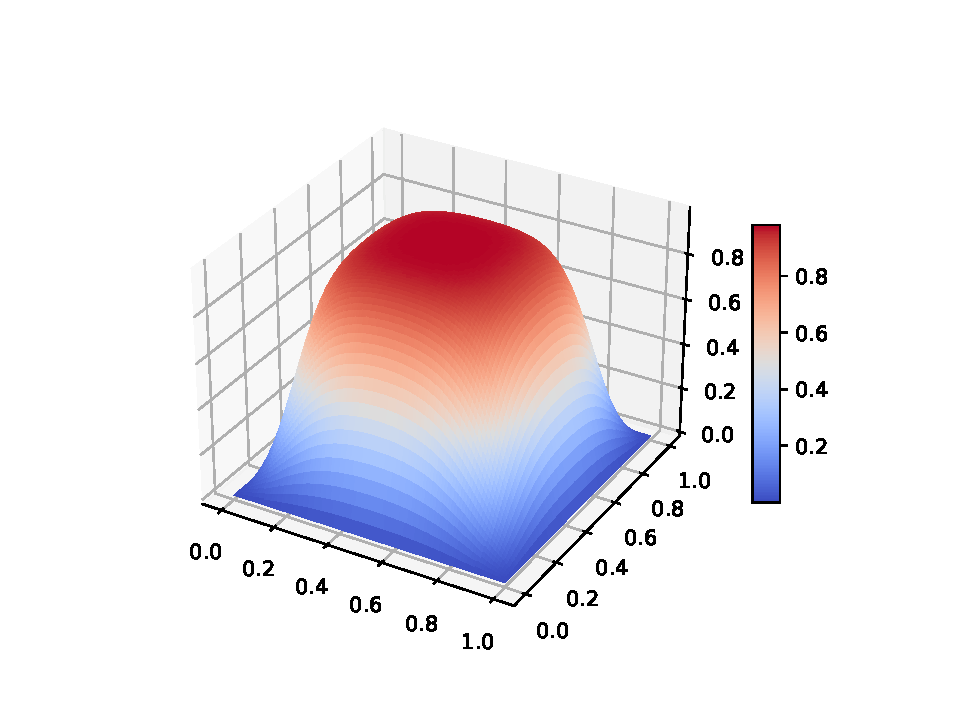
\includegraphics[width=\textwidth,height = 0.8\textwidth ]{true_pic/0.046_uh.pdf}
    \caption{\(\epsilon = 0.046\)の\(\hat{u}\)}
    \label{fi:uh_ans0.046}
  \end{minipage}
  \begin{minipage}{0.45\hsize}
    \centering
    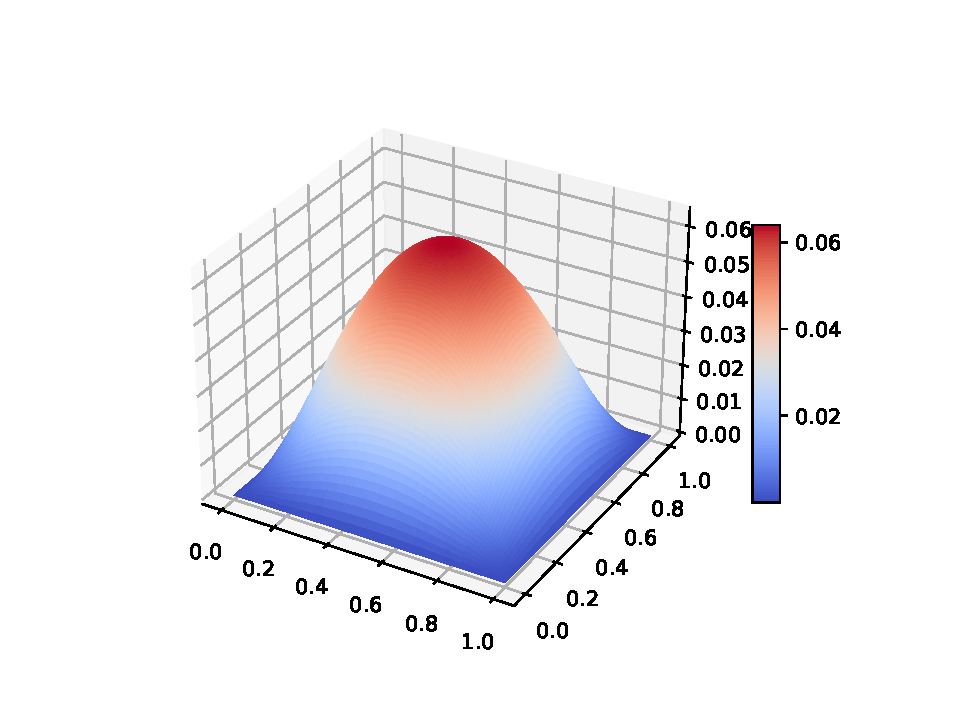
\includegraphics[width=\textwidth,height = 0.8\textwidth ]{true_pic/0.046_vh.pdf}
    \caption{\(\epsilon = 0.046\)の\(\hat{v}\)}
    \label{fi:vh_ans0.046}
  \end{minipage}\\

\end{figure}
\newpage

\begin{table}[htbp]
  \centering
  \caption{近似解に対して得られた定数}\label{hyou:定数}
  \begin{tabular}{|c|c c c|}
   \hline
   \(\epsilon\) & \(C_{h,\tilde{\mathcal{F}}}\) & \(C_{p\tilde{\mathcal{F}}}\) & \(C_{h,d}\) \\ \hline
   0.06 & 0.019781494896557579 & 0.061985811232542439 & 0.01939174236031831 \\
   0.05 & 0.019632541570461935 & 0.052066434994814518 & 0.01943154834836381 \\
   0.047 & 0.019602218508687552& 0.049294727603788044 & 0.019422869675834436 \\
   0.046 & 0.019592886535946142 & 0.048383084179607773 & 0.019419635005712356 \\\hline
  \end{tabular}
\end{table}

\begin{table}[htbp]
  \centering
  \caption{近似解に対する精度保証結果}\label{hyou:精度保証結果}
  \begin{tabular}{|c|c c c|}
   \hline
   \(\epsilon\) & \(\|-\Delta \hat{u}-f(\hat{u})+\frac{\delta}{\epsilon^2}\mathcal{B}\hat{u}\|_{L^2}\) & \(R\) & \(G\) \\ \hline
   0.06 & 3.4184815526384609e-07 & 2.1189735222377623e-08 & 1147.0626465007529 \\
   0.05 & 3.421971686405465e-06 & 1.7816986636432598e-07 & 3568.6001579986656 \\
   0.047 & 1.3774916570756025e-05 & 6.7903076012032439e-07 & 5032.2387641507731 \\
   0.046 & 1.7574433632739829e-05 & 8.5030530186178117e-07 & 5653.3462800276057 \\\hline
  \end{tabular}
\end{table}

\begin{table}[htbp]
  \centering
  \caption{\(K\) , \(K^2RG\) , \(\norm{\hat{u}-u^*}_{\tilde{\mathcal{F}}}\)の数値的検証結果}\label{hyou:数値的検証結果}
  \begin{tabular}{|c|c c c|}
   \hline
   \(\epsilon\) & \(K\) & \(K^2RG\) & \(\norm{\hat{u}-u^*}_{\tilde{\mathcal{F}}}\) \\ \hline
   0.06 & 13.64907383442583 & 0.0045281315313071549 & 2.8987805624564077e-07 \\
   0.05 & 10.848110033251072 &0.074823894310034265 & 2.0110926835478317e-06\\
   0.047 & 10.484939395162954 & 0.37564925870664212 & 9.5010307002190573e-06 \\
   0.046 & 10.386945994399487 & 0.51862831277272848 & Verification failed \\\hline
  \end{tabular}
\end{table}
